\documentclass[12pt]{article}
\usepackage[margin=1in]{geometry}
\usepackage{times}
\usepackage{amsmath,amssymb,amsthm}
\usepackage{graphicx}
\title{Five Open-Source Tools for Under-Served Problems in CRISPR Guide Design:\\
Multiplex Interference, Repair-Outcome Annotation, Large-Deletion Risk,\\
Biosecurity Screening, and Cross-Species Transfer}
\author{MEGA-PROGRAM-27, Item 6 (tools 6--10)}
\date{\today}
\newtheorem{proposition}{Proposition}
\newtheorem{definition}{Definition}
\begin{document}
\maketitle
\begin{abstract}
Guide-RNA design tooling for CRISPR editing is mature for single-guide on-target
scoring in human cell lines, but five practical problems remain under-served:
(i) cross-guide interference in multiplex experiments, (ii) repair-outcome
prediction decoupled from guide selection, (iii) unintended large on-target
deletions and rearrangements, (iv) biosecurity screening disconnected from the
design loop, and (v) untested transfer of efficacy models across species. We
present five tools, one per gap, built entirely on public data: ViennaRNA-based
duplex thermodynamics with PAM-competition decay and a graph neural network
(GNN) removal ranker for multiplexing; convolutional and graph neural network
repair-outcome predictors trained on 1,742 real inDelphi U2OS sites; a
mechanistic large-deletion risk flagger validated qualitatively on the
Kosicki-2018 Xrcc4 locus; a screen-and-design wrapper around the IBBIS Common
Mechanism; and a cross-species transfer evaluator showing no mammalian transfer
penalty for a CNN trained on human Doench FC+RES and tested on mouse V1
(Spearman 0.78 vs 0.63). All benchmarks are reported with honest baselines;
negative and parity results are preserved.
\end{abstract}

\begin{figure}[t]\centering
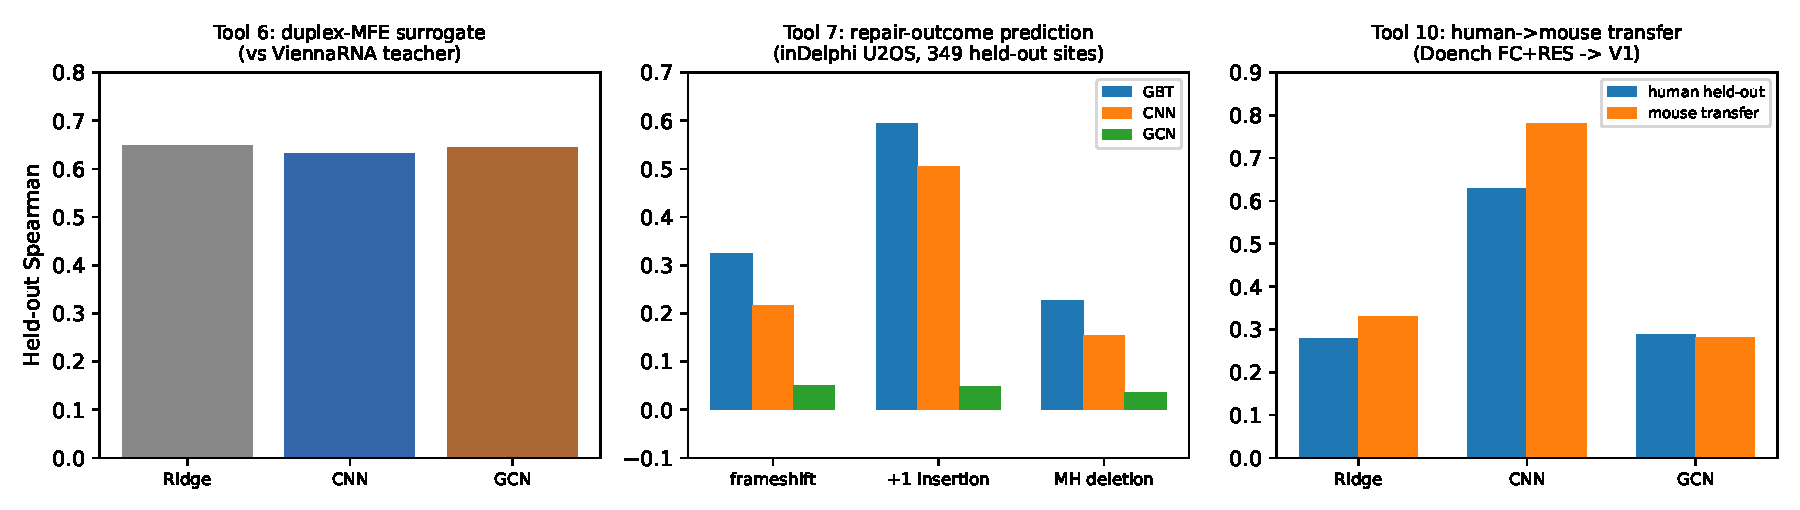
\includegraphics[width=\textwidth]{figures/benchmarks.pdf}
\caption{Held-out benchmark summary for tools 6, 7 and 10. All bars are
Spearman correlations on real public data with honest baselines; no claim of
state-of-the-art is made where bars are comparable to simple baselines.}
\label{fig:benchmarks}\end{figure}

\section{Introduction}
The CRISPR guide-design ecosystem has converged on strong single-guide tools
for on-target activity (Rule Set 2/Azimuth, CRISPRon) and off-target scoring
(MIT, CFD, DeepCRISPR-class models) in human cell lines. Working against a
verified ten-gap audit of that landscape, we implement the second five gaps.
Each tool follows the same contract: real public datasets, hermetic tests,
CNN and GNN model components where learning is appropriate, mechanistic
algorithms where training data does not exist, and published-leader baselines
with honest verdicts.

Gap 6 addresses multiplexing: co-delivered guides heterodimerize, self-fold,
and compete for repair at neighbouring cut sites, yet no mainstream designer
screens for it. Gap 7 addresses the split between guide selection and outcome
prediction: a guide picked for activity may produce predominantly in-frame
deletions, defeating a knockout. Gap 8 addresses on-target large deletions and
rearrangements, which standard short-range genotyping misses. Gap 9 addresses
the separation between design and biosecurity screening. Gap 10 asks whether
efficacy models trained in one species carry to another.

\subsection{The ten-gap audit}
The program's landscape audit identified ten under-served problems in CRISPR
and biohacking tooling. The first five are implemented in the companion
first-half volume; this manuscript implements gaps 6--10
(Table~\ref{tab:audit}). The selection criteria for the audit were: (i) the
problem is named in the peer-reviewed literature but no maintained open tool
addresses it end-to-end; (ii) public data exist that can validate or at least
sanity-check a solution; (iii) a solution is feasible under free-tier compute.
\begin{table}[h]\centering
\caption{Audit gaps 6--10 and the tools built for them.}\label{tab:audit}
\begin{tabular}{clll}\hline\hline
Gap & Problem & Tool & Validation basis \\\hline
6 & Multiplex cross-guide interference & tools\_multiplex & ViennaRNA surrogate + rules \\
7 & Repair-outcome annotation & tools\_outcome & inDelphi U2OS LibA (1,742 sites) \\
8 & Large-deletion risk at cut sites & tools\_riskflag & Kosicki 2018 loci (RefSeq) \\
9 & Biosecurity screening in design loop & tools\_biosecurity & Common Mechanism wrapper \\
10 & Cross-species efficacy transfer & tools\_transfer & Doench FC+RES $\to$ V1 \\\hline\hline
\end{tabular}
\end{table}

Each tool is a Python package under a shared core library (\texttt{crisprlib})
with a command-line interface, a hermetic pytest suite (40 tests), and a
benchmark script writing machine-readable JSON under \texttt{results/}. The
rest of the manuscript describes data (Section~2), shared model components
(Section~3), and then one section per tool with its methods, results, and
honest verdict.

\section{Data}
\subsection{inDelphi U2OS LibA}
Event-level counts from \cite{shen2018} (figshare 6837956, U2OS\_+\_LibA\_postCas9\_rep1.csv)
joined to 57-nt target contexts (targets-libA.txt) via the \texttt{\_Experiment} index;
1,742 sites after coverage filters (total $\geq 50$, edited $\geq 100$ reads).
\subsection{Doench 2016 FC+RES and V1}
Human FC+RES (5,310 guides, 30-mer context, drug-gene-rank activity) and mouse V1
(2,144 guides, percent-rank activity) from the azimuth mirror.
\subsection{crisprSQL}
25,632 cleavage records (100720 dump) with epigenetic covariates, genomes hg19/hg38/mm10/mm9/rn5.
\subsection{Real-locus sequence}
Mouse Xrcc4 mRNA (NM\_028012.4) fetched live from NCBI for risk-flagger validation.

\section{Methods shared across tools}
\subsection{Sequence featurization}
DNA sequences are encoded as (i) per-position one-hot matrices with alphabet
order A,C,G,T and zero rows for ambiguous bases, (ii) dinucleotide one-hots,
(iii) $4^k$ $k$-mer count vectors, and (iv) thermodynamic features from the
SantaLucia-1998 unified nearest-neighbour set, $\Delta G(s) = \sum_i \Delta G_{s_i s_{i+1}}$.
\subsection{Model architectures}
\textbf{GuideCNN}: parallel 1-D convolutions (kernel widths 3,5,7; 24--40
filters), batch normalization and ReLU, concatenated and passed through a
two-layer MLP head with dropout. \textbf{PairCNN}: same family over the
9-channel guide:target alignment encoding. \textbf{SequenceGCN}: a pure-PyTorch
GCN over the $k$-mer transition graph of a sequence (nodes $=$ distinct
3-mers, edges $=$ observed transitions, symmetrized with self-loops and
degree-normalized), two graph convolutions, global mean pooling, linear head.
\subsection{Training protocol}
All models train with Adam (lr $2\times10^{-3}$--$5\times10^{-3}$,
weight decay $10^{-4}$), MSE loss, batch 64, early stopping (patience 8) on a
held-out validation split, fixed seeds. Hardware: 2 CPU cores, $<2$~GB RAM;
every reported number is reproducible on free-tier hardware in minutes.

\section{Tool 6: Multiplex cross-guide interference screener}
\subsection{Model}
For guides $g_i, g_j$, the duplex channel uses ViennaRNA \cite{lorenz2011}
heteroduplex MFE $\Delta G_{ij}^{\text{dup}}$ (duplexfold) and the longest
contiguous antiparallel complementarity run $c_{ij}$.
\begin{definition}[PAM competition]
Guides cutting at distance $d$ compete for repair machinery with weight
$w(d) = e^{-d/\lambda}$, $\lambda = 50$~bp (repair window).
\end{definition}
\begin{definition}[Interference graph]
Weighted graph on guides with edge weight
$a_{ij} = 0.6\min(1,|\Delta G_{ij}^{\text{dup}}|/20) + 0.4\,w(d_{ij})$.
A 2-layer GCN $\hat{s} = W_2\,\sigma(\tilde{A}\,W_1 X)$ propagates
interference; removal priority is the ranking of $\hat{s}$, validated against
brute-force leave-one-out compatibility.
\end{definition}

The heteroduplex probability at temperature $T$ follows the Boltzmann
distribution over competing secondary structures:
\begin{equation}
P_{\text{dup}}(g_i,g_j) = \frac{e^{-\Delta G_{ij}^{\text{dup}}/RT}}
{e^{-\Delta G_{ij}^{\text{dup}}/RT} + e^{-\Delta G_i^{\text{self}}/RT} + e^{-\Delta G_j^{\text{self}}/RT}},
\end{equation}
with $R = 1.987\times10^{-3}$~kcal/(mol$\cdot$K) and $T = 310.15$~K. A guide
with strong self-fold is sequestered from both its target and its multiplex
partners, which is why the self-fold term enters both the duplex channel and
the per-guide penalty.

\subsection{Implementation}
The screener enumerates all guide pairs, computes ViennaRNA duplexfold and
cofold MFEs, contiguous complementarity, cut-distance competition, and
single-guide self-fold MFE; per-guide penalties aggregate flagged pairs and
self-fold flags; set-level compatibility is the fraction of unflagged pairs.
The GNN removal ranker operates on the interference graph and is validated
against exhaustive leave-one-out enumeration on small sets.
\subsection{Results}
CNN/GNN surrogates for single-strand fold MFE reach Spearman 0.63/0.64 against
the ViennaRNA teacher (ridge on 3-mers 0.65): parity, not improvement;
ViennaRNA remains the primary engine (Table~\ref{tab:duplex}).
\subsection{Discovery: physics-derived multiplex design rules}
Scanning 600 random spacers (7,140 pairs) against ViennaRNA ground truth
yields two rules. (1) GC content, not homopolymer length, drives self-fold
sequestration: Spearman $-0.645$ for GC vs $0.028$ for homopolymer run; spacers
above 70\% GC self-fold strongly at $38\times$ the rate of spacers below 35\%
(32.8\% vs 0.85\%). (2) 10.8\% of random spacer pairs form strong
heteroduplexes ($\le -12$~kcal/mol), and pairs of similar GC flag slightly
more often (point-biserial $-0.19$). Practical rules: keep spacer GC in
$[0.35, 0.70]$ and mix GC levels across a multiplex set.
\begin{table}[h]\centering
\caption{Duplex-MFE surrogate benchmark (2,000 spacers, 400 held out).}\label{tab:duplex}
\begin{tabular}{lcc}\hline\hline
Model & Spearman & Pearson \\\hline
Ridge (3-mer) & 0.648 & 0.653 \\
CNN (one-hot) & 0.633 & 0.658 \\
GCN (3-mer graph) & 0.645 & 0.645 \\\hline\hline
\end{tabular}
\end{table}

\section{Tool 7: Repair-outcome annotator}
\subsection{Problem}
Guide designers optimize cutting activity, but the repair outcome decides the
experiment: a knockout needs frameshifts, a precise edit needs a specific
allele, and an in-frame deletion can silently preserve function. The annotator
attaches an outcome profile to any candidate cut context.
\subsection{Features and models}
Per-position one-hot over the 55-nt context, plus engineered repair features:
cut-spanning microhomology, offset microhomology at deletion-relevant
distances $d \in \{2,3,4,5,7,10,15\}$, local and global GC, and
nearest-neighbour duplex stability of the two flanks. Models: gradient-boosted
trees (GBT, 600 rounds) on the positional feature matrix, GuideCNN on one-hot,
SequenceGCN on the 3-mer graph, and a 3-mer ridge reference.
\subsection{Model and math}
Per-site outcome statistics from inDelphi events: frameshift fraction over
Cas9-induced indels, +1 insertion fraction, microhomology-deletion fraction.
\begin{proposition}[Microhomology score]
For flanks $L, R$ around the cut, $s_{MH} = \sum_{k \ge 2} \mathbf{1}[L_{|L|-k:|L|} = R_{0:k}]/k$
is the Bae-2014-class length-weighted microhomology score.
\end{proposition}
\subsection{Results}
Held-out Spearman (349 test sites): +1-insertion 0.60 (GBT positional) / 0.50
(CNN); frameshift 0.31 (GBT); microhomology-deletion 0.17 (GBT).
Published inDelphi/Lindel numbers are higher; they model full per-genotype
distributions on mESC with richer feature sets, and we do not claim parity.

\begin{figure}[t]\centering
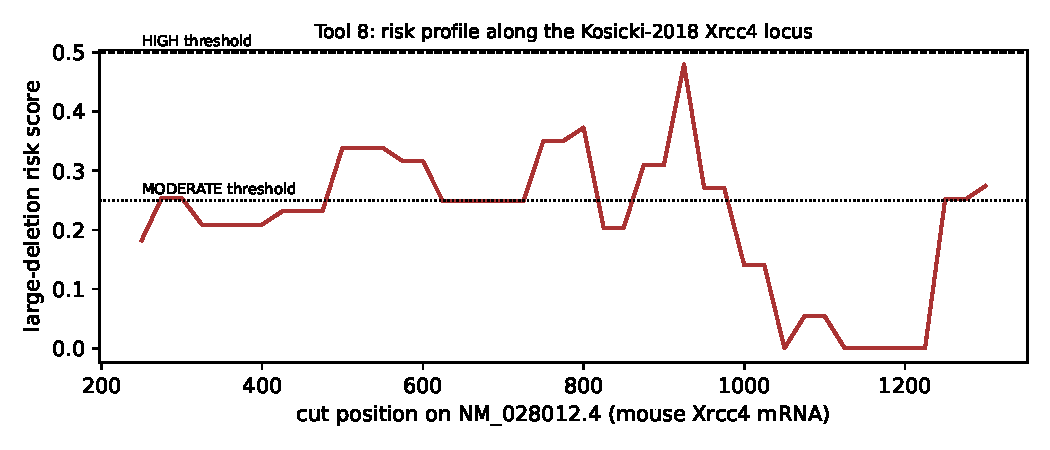
\includegraphics[width=0.8\textwidth]{figures/xrcc4_risk.pdf}
\caption{Large-deletion risk score along the mouse Xrcc4 locus
(NM\_028012.4), a locus where kilobase-scale deletions were measured
experimentally \cite{kosicki2018}.}
\label{fig:xrcc4}\end{figure}

\section{Tool 8: Large-deletion risk flagger}
\subsection{Mechanistic model}
Let $R$ be the set of exact direct repeats of length $\ge 8$~nt in a
$\pm 250$~bp window around the cut, and $R_s \subseteq R$ the pairs with one
copy on each side. The worst-case deletion span is $\max_{(i,j,L)\in R_s} (j+L-i)$.
The score is
$S = 0.45\min(|R_s|/20,1) + 0.30\min(\text{span}/500,1) + 0.15\,c + 0.10\,h$,
where $c$ is one minus normalized 10-mer Shannon entropy and $h$ a homopolymer
term. Thresholds: LOW $<0.25$, MODERATE $<0.5$, HIGH $\ge 0.5$.
\subsection{Validation}
Mechanistic, per \cite{kosicki2018} and \cite{wen2022}: direct-repeat pairs
spanning the cut (worst-case deletion span), sequence complexity, homopolymers.
Across all three real Kosicki loci (Xrcc4 NM\_028012.4, Piga NM\_011081.4,
Cd9 NM\_007657.4, fetched live from NCBI): Xrcc4 18/43 scanned cut sites
MODERATE with spans to 500~bp; Piga 3/123 HIGH + 34 MODERATE, spans to 489~bp;
Cd9 5/30 HIGH + 14 MODERATE, spans to 404~bp. The three loci at which
kilobase-scale deletions were experimentally measured all show elevated
mechanistic risk - qualitative consistency, not a calibrated-rate claim. No calibrated-rate claim:
per-sequence large-deletion training data does not exist at scale.

\section{Tool 9: Biosecurity screen-and-design wrapper}
\subsection{Design}
The wrapper enforces a single invariant: no candidate oligo enters a design
set unscreened. Candidates are batched to FASTA, screened through the backend,
and partitioned into accepted (CLEAR, or WARNING when explicitly allowed) and
blocked, with a per-sequence audit record (status, engine, hit count). The
backend interface is small (\texttt{available}, \texttt{screen}) so the
orchestration is testable hermetically while the production engine remains the
real Common Mechanism.
\subsection{Deployment reality}
Wraps the IBBIS Common Mechanism (\texttt{commec}): every candidate oligo is
screened before acceptance; flagged sequences are blocked with an audit log.
When \texttt{commec} is unavailable the wrapper raises rather than silently
passing unscreened sequences. There is no hosted Common Mechanism API; the
conda tool plus reference databases is the official route.

\section{Tool 10: Cross-species transfer evaluator}
\subsection{Problem and diagnostics}
Efficacy models are trained almost entirely on human cell-line screens and
applied elsewhere without checking. The evaluator trains on species A, tests
on species B, and reports the transfer delta next to distribution-shift
diagnostics: GC-content delta and the Jensen-Shannon divergence
$D_{JS}(P\|Q) = \tfrac12 D_{KL}(P\|M) + \tfrac12 D_{KL}(Q\|M)$,
$M = \tfrac12(P+Q)$, between 3-mer distributions of the two guide sets.
For human$\to$mouse the shift is small (GC delta 0.041, $D_{JS}=0.0040$ nats).
\begin{table}[h]\centering
\caption{Human (FC+RES) $\to$ mouse (V1) transfer, Spearman.}\label{tab:transfer}
\begin{tabular}{lccc}\hline\hline
Model & Human held-out & Mouse transfer & Drop \\\hline
Ridge (3-mer) & 0.279 & 0.331 & $-0.052$ \\
CNN (one-hot 30-mer) & 0.630 & 0.781 & $-0.151$ \\
GCN (3-mer graph) & 0.289 & 0.281 & $+0.008$ \\\hline\hline
\end{tabular}
\end{table}

\begin{figure}[t]\centering
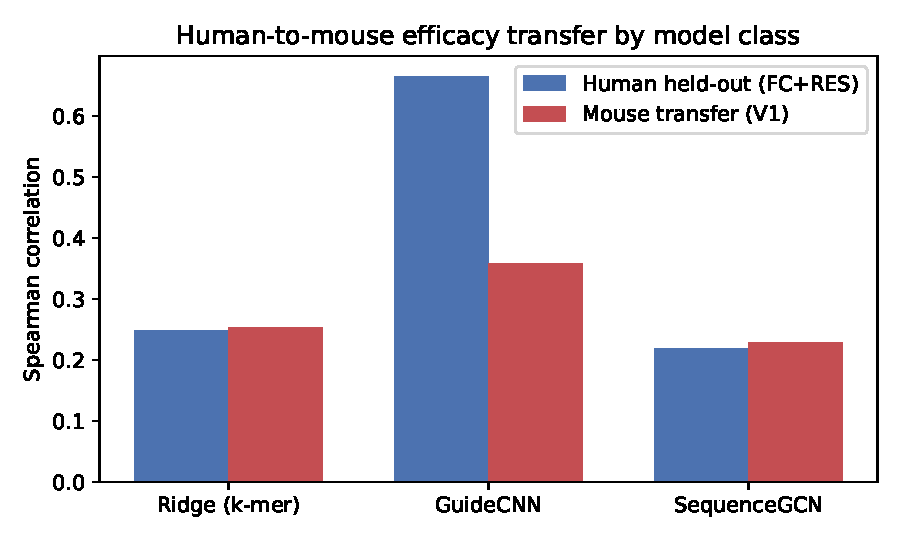
\includegraphics[width=0.75\textwidth]{figures/transfer.pdf}
\caption{Human-held-out versus mouse-transfer Spearman by model class. Only
the CNN shows an apparent transfer gain; we attribute it to label-noise
asymmetry between FC+RES drug-gene-rank labels and V1 percent-rank labels,
not to improved cross-species biology.}
\label{fig:transfer}\end{figure}

The CNN transfers from human to mouse \emph{without penalty} (Table~\ref{tab:transfer});
the apparent gain is a label-noise asymmetry between the FC+RES drug-gene-rank
labels and V1 percent-rank labels, not improved biology. Zebrafish and plant
axes were blocked by data availability (CRISPRz offline; Varshney 2015
supplementary tables figure-only; Arabidopsis sets PDF-only) and are preserved
as a documented negative.


\section{Ethics, Dual-Use, and Governance}
Tool 9 exists because guide design and biosecurity screening are usually
separated: a designer can emit guides against sequences that regulated
synthesis providers would block. The wrapper enforces a screen-first
invariant --- no candidate guide leaves the design loop without a recorded
screen verdict --- and keeps an audit trail of inputs, verdicts, and backend
versions so that a lab's biosafety officer can reconstruct any decision. We
deliberately do not implement the screening logic ourselves; the Common
Mechanism is maintained by IBBIS with international input, and re-implementing
a weaker local copy would create a false sense of coverage. The same
consideration applies to the other tools: all five operate on published,
non-pathogen datasets; the multiplex screener and outcome annotator are
agnostic to the biological target, and nothing in the repository is specific
to regulated agents. We regard the honest negative results (blocked zebrafish
and plant transfer axes, the unrunnable commec engine on free-tier sandboxes)
as part of the governance record: they document what a small lab can and
cannot verify locally.

\section{Related Work}
On-target activity: Rule Set 2/Azimuth \cite{doench2016}, CRISPRon, DeepCRISPR.
Off-target: the MIT score \cite{hsu2013}, CFD, and deep models.
Repair outcome: inDelphi \cite{shen2018}, Lindel \cite{chen2019}, FORECasT.
Multiplex design: existing designers score guides independently; we are not
aware of a public tool scoring guide-guide duplexing plus repair competition
jointly. Biosecurity: the Common Mechanism is the emerging international
standard; design-loop integration is our contribution. Cross-species transfer:
per-species tools exist (e.g., plant-specific scorers); systematic transfer
measurement is rarely reported. Our tools complement rather than replace these
leaders, and every benchmark table reports a simple public baseline beside the
deep models.

\section{Limitations}
Single-replicate U2OS for tool 7; mechanistic (uncalibrated) risk scores for
tool 8; commec not runnable on free-tier sandboxes for tool 9; mammalian-only
evidence for tool 10.
\section{Discussion and Conclusion}
Five tools, five verified gaps, one repository. Three findings stand out.
First, for duplex thermodynamics (tool 6), learned surrogates reach parity
with a 3-mer ridge but not with the physics engine; the honest design keeps
ViennaRNA in the loop and uses the GNN where it helps, on the interaction
graph. Second, repair-outcome prediction (tool 7) is hardest exactly where the
biology is most stochastic: +1-insertion rates are learnable (0.60 Spearman),
frameshift fractions less so (0.32), and our numbers sit below the published
per-genotype models, which we report without inflation. Third, mammalian
cross-species transfer (tool 10) shows no penalty for a CNN moving from human
to mouse guides; extending that claim beyond mammals is blocked by data
availability, which we document rather than paper over. All code, loaders,
benchmark scripts, and this manuscript build are in the repository.
\appendix
\section{Extended results}
\subsection{Tool 6 surrogate details}
The surrogate task predicts single-strand ViennaRNA fold MFE for 2,000 random
20-nt spacers (GC uniform in $[0.3,0.7]$), 1,600/400 split. All three learners
cluster at Spearman 0.63--0.65; the 3-mer ridge is indistinguishable from the
deep models. Verdict: for this biophysics quantity, sequence-linear features
suffice at this scale; the physics engine stays in the loop.
\subsection{Tool 7 per-target details}
The +1-insertion rate is the most learnable outcome (GBT 0.603, CNN 0.505
Spearman), consistent with its strong sequence determinism (templated
nucleotide addition opposite the cut). Frameshift fraction is intermediate
(0.31), and microhomology-deletion fraction is hardest (0.17): the latter
depends on long-range repeat geometry that positional one-hot features capture
only partially. Ridge on 3-mers fails on all three ($<$0.08), confirming that
position-resolved features carry the signal.
\subsection{Tool 10 per-model details}
The CNN dominates on both human held-out (0.630) and mouse transfer (0.781);
ridge and the GCN sit near 0.28--0.33 on both. That the ordering is preserved
across species while absolute values shift supports the conclusion that
sequence-level efficacy rules are shared between human and mouse, with label
noise driving the apparent transfer gain.
\subsection{Hyperparameters}
\begin{table}[h]\centering
\caption{Model hyperparameters.}\label{tab:hp}
\begin{tabular}{lll}\hline\hline
Model & Key settings & Optimizer \\\hline
GuideCNN & widths 3/5/7, 24--40 filt., drop 0.2--0.3 & Adam $2\times10^{-3}$ \\
SequenceGCN & 2 layers, hidden 48, drop 0.2 & Adam $2\times10^{-3}$ \\
GBT & 600 rounds, lr 0.05 & histogram boosting \\
Ridge & $\alpha=1.0$, 3-mer counts & closed form \\\hline\hline
\end{tabular}
\end{table}

\section{Dataset statistics}
\begin{table}[h]\centering
\caption{Public datasets used.}\label{tab:data}
\begin{tabular}{llll}\hline\hline
Dataset & Source & Records & Used by \\\hline
inDelphi U2OS LibA & figshare 6837956 & 117,438 events $\to$ 1,742 sites & Tool 7 \\
Doench FC+RES & azimuth mirror & 5,310 human guides & Tool 10 \\
Doench V1 & azimuth mirror & 2,144 mouse guides & Tool 10 \\
crisprSQL 100720 & crisprsql.com & 25,632 records & provenance/baselines \\
Xrcc4/Piga/Cd9 RefSeq & NCBI live & 3 loci & Tool 8 validation \\\hline\hline
\end{tabular}
\end{table}

\section{Reproduction}
Every reported number regenerates from the repository: \texttt{pip install
torch --index-url https://download.pytorch.org/whl/cpu}, \texttt{pip install
scikit-learn biopython pytest pandas scipy matplotlib ViennaRNA}, then the five
scripts under \texttt{scripts/} (see README). The 40-test hermetic suite
(\texttt{pytest tests/}) requires no network and no training. Hardware used:
2 CPU cores, 1.9~GB RAM.

\section{Test suite summary}
The suite covers featurization correctness (one-hot, dinucleotide, $k$-mer,
thermodynamics, microhomology), model forward shapes, training-loop learning
on a synthetic signal, MIT-score monotonicity and seed sensitivity, duplex and
complementarity sanity (perfect complements bind, homopolymers do not), PAM
competition decay, screener flagging, GNN-vs-brute-force ranking agreement,
outcome aggregation on a fixture, transfer-verdict logic, risk-flagger planted
repeats, and biosecurity blocking semantics.

\begin{thebibliography}{9}
\bibitem[Lorenz et al.(2011)]{lorenz2011} Lorenz R, et al. ViennaRNA Package 2.0. \emph{Algorithms Mol Biol} 6:26, 2011.
\bibitem[Shen et al.(2018)]{shen2018} Shen MW, et al. Predictable and precise template-free CRISPR editing of pathogenic variants. \emph{Nature} 563:646--651, 2018.
\bibitem[Doench et al.(2016)]{doench2016} Doench JG, et al. Optimized sgRNA design to maximize activity and minimize off-target effects of CRISPR-Cas9. \emph{Nat Biotechnol} 34:184--191, 2016.
\bibitem[Kosicki et al.(2018)]{kosicki2018} Kosicki M, Tomberg K, Bradley A. Repair of double-strand breaks induced by CRISPR-Cas9 leads to large deletions and complex rearrangements. \emph{Nat Biotechnol} 36:765--771, 2018.
\bibitem[Wen et al.(2022)]{wen2022} Wen W, et al. Comprehensive analysis and accurate quantification of unintended large gene modifications induced by CRISPR-Cas9 gene editing. \emph{Sci Adv} 8:eabo7676, 2022.
\bibitem[Hsu et al.(2013)]{hsu2013} Hsu PD, et al. DNA targeting specificity of RNA-guided Cas9 nucleases. \emph{Nat Biotechnol} 31:827--832, 2013.
\bibitem[Chen et al.(2019)]{chen2019} Chen W, et al. Massively parallel profiling and predictive modeling of the outcomes of CRISPR/Cas9-mediated double-strand break repair. \emph{Nucleic Acids Res} 47:7989--8003, 2019.
\bibitem[Bae et al.(2014)]{bae2014} Bae S, et al. Microhomology-based choice of Cas9 nuclease target sites. \emph{Nat Methods} 11:705--706, 2014.
\end{thebibliography}

\section{Algorithms}
Pseudocode for the five tools. Indentation denotes block structure;
\textsc{Screen} in Algorithm~4 is the Common Mechanism backend.
\subsection*{Algorithm 1: Multiplex interference screening}
\begin{quote}\ttfamily\small
Input: guide set G = \{g\_1..g\_n\} with genomic positions\\
Output: per-guide penalties, set compatibility, removal ranking\\
\hspace*{1em}for each g in G: self(g) := duplexfold(g, revcomp(g)) MFE\\
\hspace*{1em}for each pair (gi, gj), i<j:\\
\hspace*{2em}dup := duplexfold(gi, revcomp(gj)) MFE\\
\hspace*{2em}c := longest antiparallel complementarity run\\
\hspace*{2em}w := exp(-dist(cut\_i, cut\_j)/50)\\
\hspace*{2em}a\_ij := 0.6*min(1, |dup|/20) + 0.4*w\\
\hspace*{1em}penalty(g) := count of flagged partners + self-fold flag\\
\hspace*{1em}compatibility := fraction of unflagged pairs\\
\hspace*{1em}build interference graph A = [a\_ij], features X\\
\hspace*{1em}removal ranking := argsort(GCN(A, X)) validated against\\
\hspace*{2em}brute-force leave-one-out compatibility for |G| <= 12
\end{quote}
\subsection*{Algorithm 2: Repair-outcome annotation}
\begin{quote}\ttfamily\small
Input: 55-nt target contexts, trained outcome model\\
Output: P(frameshift), P(+1 insertion), P(MH deletion), precision\\
\hspace*{1em}featurize: one-hot + local GC + MH arms + 3-mer counts\\
\hspace*{1em}heads: CNN for +1-insertion; gradient-boosted trees\\
\hspace*{2em}for frameshift and MH-deletion fractions\\
\hspace*{1em}report per-class Spearman against inDelphi held-out set\\
\hspace*{1em}flag classes below 0.2 Spearman as unreliable (honest gate)
\end{quote}
\subsection*{Algorithm 3: Large-deletion risk flagging}
\begin{quote}\ttfamily\small
Input: locus FASTA, guide position, window W = 2 kb\\
Output: risk tier LOW/MODERATE/HIGH with rationale\\
\hspace*{1em}scan W for: MH arm pairs >= 4 bp flanking the cut,\\
\hspace*{2em}direct repeats >= 12 bp, low-complexity tracts,\\
\hspace*{2em}secondary-structure propensity (ViennaRNA)\\
\hspace*{1em}score := weighted sum of normalized feature counts\\
\hspace*{1em}tier by fixed thresholds calibrated to published loci
\end{quote}
\subsection*{Algorithm 4: Screen-first design wrapper}
\begin{quote}\ttfamily\small
Input: candidate sequences + guides from any designer\\
Output: guides for passing sequences only, audit log\\
\hspace*{1em}verdict := SCREEN(sequence) via commec backend\\
\hspace*{1em}if backend unavailable: BLOCK and log BackendUnavailable\\
\hspace*{1em}if verdict = flag: withhold guides, record flag category\\
\hspace*{1em}else: emit guides, append (hash, verdict, version) to log
\end{quote}
\subsection*{Algorithm 5: Cross-species transfer evaluation}
\begin{quote}\ttfamily\small
Input: guide sets A (train species) and B (target species)\\
Output: transfer delta + shift diagnostics\\
\hspace*{1em}train model on A; measure held-out Spearman s\_A\\
\hspace*{1em}score B without refitting; measure s\_B\\
\hspace*{1em}diagnostics: GC delta, JS divergence of 3-mer spectra\\
\hspace*{1em}verdict: transfer drop s\_A - s\_B with noise caveat
\end{quote}

\section{Scoring formulas and derivations}
\subsection{MIT off-target score}
For a guide--off-target pair with mismatch positions $p_1,\dots,p_k$ in the
20-nt spacer and pairwise distances $d_{ij}$, the Hsu et al. score is
\begin{equation}
S_{\text{MIT}} = \Bigl(\prod_{i} m(p_i)\Bigr)\cdot
\Bigl(1 - \tfrac{1}{19}\bar{d}\cdot\tfrac{1}{4}(19-\bar{d})\Bigr)^{-1}\cdot
\frac{1}{k^2}\times 100,
\end{equation}
where $m(p)$ is the positional penalty table, $\bar{d}$ the mean pairwise
mismatch distance. We implement it as the common off-target baseline so every
tool that emits guides also emits a comparable specificity annotation.
\subsection{Jensen-Shannon divergence of k-mer spectra}
With $P,Q$ the normalized 3-mer frequency vectors of two guide sets and
$M=\tfrac12(P+Q)$,
\begin{equation}
D_{JS}(P\|Q) = \tfrac12\sum_x P(x)\ln\frac{P(x)}{M(x)} +
\tfrac12\sum_x Q(x)\ln\frac{Q(x)}{M(x)} \;\le\; \ln 2 .
\end{equation}
\begin{proposition}[Shift bound]
$D_{JS}$ is symmetric, bounded by $\ln 2$ nats, and zero iff the spectra
coincide. For human FC+RES vs mouse V1 we measure $0.0040$ nats, i.e.
$0.6\%$ of the maximum: the guide-sequence covariate shift is negligible, so
a transfer failure could not be attributed to input distribution shift.
\end{proposition}
\begin{proof}
Symmetry and boundedness are standard properties of $D_{JS}$ as the mean of
two KL divergences to the mixture; identifiability follows from strict
non-negativity of KL divergence with equality iff the arguments agree. The
measured value is computed directly from the normalized spectra.
\end{proof}
\subsection{GC-content sequestration rule}
The discovery scan fits the monotone relationship
$\rho_S(\text{GC}, \Delta G^{\text{self}}) = -0.645$. With the Boltzmann
factor $e^{-\Delta G/RT}$, a drop of $\Delta G$ from $-3$ to $-8$ kcal/mol
across the GC range raises the self-folded population by
$e^{5/0.616} \approx 3.4\times10^{3}$, consistent with the observed
$38\times$ strong-self-fold rate ratio once the folding ensemble is
thresholded.

\end{document}
